% ------------------------------------------------
% Week 4 research report. Built on week4/paper/template/template.tex.
% Every number traces to a file in week4/results/.
% ------------------------------------------------

\documentclass[11pt]{article}

% ------------------------------------------------
% Packages
% ------------------------------------------------
\usepackage{amsmath, amssymb}
\usepackage{graphicx}
\usepackage{hyperref}
\usepackage[numbers,square,comma,sort&compress]{natbib} % IEEE-style numeric citations
\usepackage{geometry}        % For adjusting margins
\usepackage{float}           % For controlling float positions
\usepackage{booktabs}        % For professional-looking tables
\usepackage{caption}
\usepackage{subcaption}
\usepackage{color}

% ------------------------------------------------
% Page Setup
% ------------------------------------------------
\geometry{margin=1in}
\graphicspath{{figures/}}
\newcommand{\arm}[1]{\texttt{#1}}

% ------------------------------------------------
% Title and Author Information
% ------------------------------------------------
\title{\textbf{Do Tabular Foundation Models Help the Worst-Off Group? TabPFN, Group DRO and Their Combination for Predicting Bank Account Ownership in Kenya, Rwanda, Tanzania and Uganda}}
\author{
  Charis Opol\thanks{Corresponding author: \texttt{charisopol@gmail.com}} \\
  \normalsize AI Studio Uganda \\
  \and
  Alexander Gimei \\
  \normalsize AI Studio Uganda \\
}
\date{\today}

% ------------------------------------------------
% Document Begins
% ------------------------------------------------
\begin{document}

\maketitle

% ------------------------------------------------
% Abstract
% ------------------------------------------------
\begin{abstract}
Pooled accuracy can hide which group a model fails. We test whether two routes to a fairer classifier improve performance for the worst-off country when predicting bank account ownership from 23,524 household survey responses in Kenya, Rwanda, Tanzania and Uganda. The model-side route is TabPFN v2, a pretrained tabular foundation model used without tuning. The training-side route is Group DRO with country as the group. We also test two hybrids that combine them, and evaluate every method when a whole country is held out. Six hypotheses and their falsification rules were pre-registered. Evaluation uses nested cross-validation over five seeds, out-of-fold PR-AUC and paired stratified bootstrap intervals.

TabPFN matches tuned XGBoost on pooled PR-AUC (0.590 against 0.588) with no tuning, but leaves the gap between pooled and worst-country PR-AUC unchanged. Group DRO lowers worst-country PR-AUC by 0.017 and pooled PR-AUC by 0.040. Its logged group weights show why: it concentrates on the country with the highest training loss (Kenya), not the country with the lowest PR-AUC (Rwanda). When redirected to Rwanda through within-country class weights, Rwanda's PR-AUC still does not move. No hybrid beats the better of its parents, and no method is consistently best under leave-one-country-out evaluation. The worst-off country is Rwanda, not Uganda, and its PR-AUC stays between 0.44 and 0.47 across every model and objective. For this task, the limit on serving the worst-off country appears to lie in the data rather than in the choice of model or training objective.
\end{abstract}

\vspace{0.5cm}
\noindent\textbf{Keywords:} financial inclusion, worst-group performance, TabPFN, Group DRO, distribution shift, East Africa

% ------------------------------------------------
% Main Content
% ------------------------------------------------

% 1. Introduction
\section{Introduction}

Account ownership is ``the fundamental measure of financial inclusion'' \citep[p.~27]{demirguckunt2022findex}. Machine learning has been used to predict it from household survey features, including on the dataset studied here \citep{ismail2021using, balde2022efficient}. Those studies report pooled accuracy or F1. A pooled score says little about the group for which a poor model does the most harm: the group least likely to be correctly identified, and so least likely to be reached by outreach. We take a mini-max, or Rawlsian, view and judge a model by the performance of its worst group \citep[pp.~4--5]{barrainkua2025preserving}.

There are two plausible routes to a model that serves the worst-off group better. On the model side, TabPFN v2 is a transformer pretrained on synthetic datasets that predicts by in-context learning, and is reported to beat tuned gradient-boosted trees on small tabular datasets \citep{hollmann2025accurate}. If it generalises better from few examples, it might help a small, low-prevalence country most. On the training side, Group DRO minimises the loss of the worst group rather than the average loss \citep{ghosal2023distributionally, stahlschmidt2024domain}.

The evidence for each route is mixed. Independent benchmarks find tabular foundation models roughly level with established methods \citep{shaktah2026established}, and a recent review concludes that fairness needs an explicit intervention beyond pretraining \citep[pp.~22--23]{kurashkin2026current}. On the WILDS benchmark, Group DRO generally does not beat empirical risk minimisation (ERM), and where it wins it matches simple reweighting \citep[pp.~20--22, 92]{koh2021wilds}. In the literature we reviewed, we found no study that combines a tabular foundation model with group-robust training, none that evaluates worst-group PR-AUC, and none that analyses these four countries separately or under leave-one-country-out shift.

\paragraph{Research questions.}
\begin{itemize}
  \item \textbf{RQ1.} Does TabPFN v2, out of the box, match or beat tuned XGBoost and a PyTorch MLP on pooled PR-AUC?
  \item \textbf{RQ2.} How large is the gap between pooled and worst-country PR-AUC, and does TabPFN narrow it relative to XGBoost?
  \item \textbf{RQ3.} Does Group DRO improve worst-country PR-AUC over ERM, at what pooled cost, and does it beat inverse-frequency reweighting?
  \item \textbf{RQ4.} Does any combination of TabPFN with group-robust training beat both parents on worst-country PR-AUC?
  \item \textbf{RQ5.} Training on three countries and testing on the fourth, is any method consistently best?
  \item \textbf{RQ6.} Do SHAP-measured drivers differ by country beyond resampling noise, and does Group DRO change them for the worst-off country?
\end{itemize}

\paragraph{Contributions.}
\begin{enumerate}
  \item A pre-registered, leakage-checked benchmark of TabPFN v2, XGBoost, MLPs, Group DRO and two TabPFN hybrids on worst-country PR-AUC, including an exact reproduction of an earlier baseline.
  \item Evidence from logged group weights of why Group DRO fails here: the worst group by training loss differs from the worst group by PR-AUC, and correcting the target does not help.
  \item Evidence that worst-country PR-AUC barely moves across all the model families and objectives tested.
  \item A size-matched resampling-noise baseline for comparing SHAP feature rankings between countries.
\end{enumerate}

Section~\ref{sec:related} reviews related research. Section~\ref{sec:method} describes the methods and Section~\ref{sec:experiments} the data and experimental design. Section~\ref{sec:results} reports results by research question, and Section~\ref{sec:discussion} interprets them and states the limitations.

% 2. Related Research
\section{Related Research}
\label{sec:related}

This section reviews five lines of work that bear on our questions: machine learning for financial inclusion, the long-running comparison between tree ensembles and deep networks on tabular data, tabular foundation models, group-robust and fair learning under distribution shift, and cross-group explanation. It closes by stating the gap this study addresses.

\subsection{Machine learning for financial inclusion}

The Global Findex Database calls account ownership ``the fundamental measure of financial inclusion'' and reports that ownership reached 76\% of adults worldwide and 55\% in Sub-Saharan Africa by 2021, largely through mobile money in that region \citep[pp.~20, 27]{demirguckunt2022findex}. It also documents wide gaps by gender, income, education and rural residence. For the countries in our data, it reports rural-urban gaps of 12 to 14 percentage points in Kenya, Tanzania and Uganda, and names documentation and distance as leading barriers for the unbanked in Tanzania and Uganda \citep[pp.~47, 53--54]{demirguckunt2022findex}. Findex's ``account'' includes mobile money \citep[p.~33]{demirguckunt2022findex}, a definition broader than the \texttt{bank\_account} label used here.

Two earlier studies applied machine learning to what appears to be the same Zindi dataset. \citet{ismail2021using} compared twelve classifiers on a single holdout split. XGBoost had the best accuracy (89.23\%), but its F1 was only 0.51 with recall 0.39, so the high accuracy reflects the class imbalance. They tried resampling and abandoned it because it lowered accuracy, and ranked education level as the most important feature by random-forest importance. \citet{balde2022efficient} applied SMOTE and compared nine classifiers on a 90/10 holdout, reporting about 91.5\% for random forest on accuracy, precision, recall and F1 alike. The near-identical values suggest evaluation on an oversampled test set, although the paper does not state the order of oversampling and splitting. Neither study reports per-country results or a ranking metric such as PR-AUC at the natural prevalence, and the two describe the data's origin differently \citep{ismail2021using, balde2022efficient}.

Other work studies financial access from different data. \citet{engelmann2018unbanked} predicted area-level socio-economic status in Dar es Salaam from mobile-money and call records, finding that mobile-money features raised accuracy from 65.9\% to 71.3\%, and emphasised that mobile money stands in for bank accounts for many East Africans. \citet{chen2026evaluating} predicted a Findex-derived inclusion score across 56 emerging economies with a hybrid tree and deep model, and reported region-specific SHAP signs for digital literacy, positive in Africa and Latin America and marginally negative in parts of Asia. The author describes the findings as correlational, and inconsistencies between its reported tables call for caution. In credit, \citet{shan2026tabpfn} used TabPFN v2 to predict risk for 1,050 observations of small automotive suppliers and found the best point estimates against tuned tree ensembles, but with wide intervals on only 22 positive test cases. \citet{pathan2026intelligent} averaged the probabilities of a neural network and TabPFN to predict bank customer churn. These studies show that tabular foundation models are reaching finance applications, but none examines performance for the worst-off group.

\subsection{Tree ensembles and deep learning on tabular data}

Gradient-boosted trees have long been the reference method for tabular data. XGBoost combines a regularised objective, a second-order approximation, shrinkage and column subsampling with sparsity-aware split finding and a scalable system design \citep{chen2016xgboost}. \citet{shwartzziv2021tabular} compared four deep tabular architectures with XGBoost under the same tuning protocol on eleven datasets. Each deep model did best mainly on the datasets from its own paper, XGBoost generally won on unseen datasets with less tuning, and an ensemble of both performed best. They warned that reported deep-learning gains may reflect selection bias and unequal tuning. The survey of \citet{borisov2024deep} reached a similar conclusion: tree ensembles still mostly win on small and medium datasets, and deep models lag except on a very large, mostly numeric dataset. They attribute this to heterogeneous features, the lack of spatial structure, dependence on preprocessing and the importance of single features. \citet{jiang2026representation} survey representation learning for tabular data and state that rigorous benchmarking against established non-deep methods ``remains a critical standard''. These findings shaped our design: we tune XGBoost and the MLP within a nested loop with the same budget, and treat XGBoost as the baseline that any new method must match.

\subsection{Tabular foundation models}

\paragraph{TabPFN.} TabPFN v2 is a transformer pretrained on about 130 million synthetic datasets drawn from structural causal models. It predicts on a new dataset by in-context learning in a single forward pass, approximating the posterior predictive distribution given the labelled training rows as context \citep[p.~2]{hollmann2025accurate}. Attention runs over both features and samples, and test rows attend only to training rows. On benchmarks of up to 10,000 samples and 500 features, default TabPFN beat tuned gradient-boosted trees and AutoGluon on normalised ROC AUC at much lower time cost. Its authors state that these results ``should not be taken as evidence that TabPFN scales well beyond the 10,000 samples and 500 features'' \citep[p.~6]{hollmann2025accurate}. The paper also demonstrates embeddings taken from the final layer, fine-tuning and SHAP support, but does not address fairness or group robustness. Later versions extend the size envelope \citep{jiang2026representation, kurashkin2026current}.

\paragraph{Independent evaluations.} Evidence from outside the original authors is more mixed. \citet{shaktah2026established} benchmarked TabPFN v2.5 against twelve established classifiers on twelve clinical tasks. TabPFN beat the best established model in only 2 of 12 tasks, most AUROC differences lay within $\pm 0.02$, and its median runtime was 5.53 times longer, so the authors recommend treating it as a complement rather than a replacement. \citet{costa2026high} found that tabular foundation models reach the highest AUC on 112 datasets but have weaker size-stratified conditional coverage than gradient-boosted trees, a sign of overconfident errors that worsens under high noise. \citet{sabanovic2026calibration} found TabPFN v2's raw probabilities already well calibrated on its compatible datasets. For regression, \citet{johnson2026uncertainty} found no consistent winner between TabPFN and Gaussian processes and no meaningful gain from tuning TabPFN beyond its defaults, which supports evaluating it out of the box. The critical review of \citet{kurashkin2026current}, covering 98 studies, concludes that in-context prediction works but that independent evidence has not matched benchmark claims. It finds these models strongest on small to medium independent and identically distributed data, with tuned trees or deep models the safer default under grouped or non-IID shift, and treats calibration, robustness and fairness as properties of the surrounding pipeline rather than of the forward pass \citep[pp.~22--23]{kurashkin2026current}.

\paragraph{Context and fine-tuning.} Because a foundation model makes no weight updates at prediction time, the choice of context rows carries much of the weight that hyperparameters once did \citep[p.~19]{kurashkin2026current}. Several studies exploit this. \citet{djilani2026robustness} showed that changing only the context improved TabPFN's adversarial robustness more than fine-tuning its weights, and subsampled large datasets to a 10,000-row context. \citet{fieggen2025navigating} kept all positives and sampled negatives to fit a rare-disease dataset into TabPFN's context, a precedent for prevalence-altering subsampling, and found TabPFN reached high AUC whereas SMOTE harmed XGBoost. On fine-tuning, \citet{tanna2026exploring} compared zero-shot inference, meta-learning, full supervised fine-tuning and parameter-efficient fine-tuning across six foundation models. Zero-shot was already strong, full fine-tuning often hurt accuracy and calibration although TabPFN tolerated it best, gains were largest on medium-sized or wide datasets, and fairness showed an accuracy-equity trade-off. \citet{jiang2026representation} instead report that fine-tuning typically improves on zero-shot inference. Our H1 hybrid follows the context-design line, and the infeasibility of H3 reflects how little support current software offers for custom fine-tuning objectives.

\subsection{Tabular foundation models across groups and under shift}

Few studies ask how tabular foundation models behave across groups. \citet{das2026bridging} studied genomic risk prediction for under-sampled ancestry groups. Off-the-shelf TabPFN degraded less than elastic net and random forest under sample imbalance, but failed when effect sizes varied across ancestries, and only a version instruction-tuned on synthetic non-stationary tasks became more stable for individuals far from the context. This separation of a sample-size effect from a changing-relationship effect is the closest analogue in our literature to the question of why one country is worst served. \citet{harijeyan2025evaluating} trained on one demographic subgroup of the Adult dataset and tested on another, finding XGBoost strongest in distribution and TabPFN highest or near-highest out of distribution, although the baselines appear untuned. \citet{liu2026causal} evaluated TabPFN on four fairness benchmarks under varying size, spurious correlation and missing-not-at-random shift. It had strong accuracy, but its gains in demographic parity and equalised odds were moderate and inconsistent, and the authors conclude that causal pretraining is helpful but insufficient for fairness. \citet{guan2026stablepfn} showed that a structural change to the model, masking attention to a discovered Markov boundary, improves stability across environments for regression under an invariance assumption. Together these studies suggest that pretraining alone does not guarantee good performance for every group, which motivates pairing TabPFN with an explicit group-robust method.

\subsection{Group robustness and fairness under distribution shift}

\paragraph{Worst-group objectives.} \citet{barrainkua2025preserving} survey methods that keep fairness guarantees when training and deployment distributions differ. They define mini-max, or Rawlsian, fairness as minimising the error of the worst-off group \citep[pp.~4--5]{barrainkua2025preserving}, distinguish demographic, covariate, label, concept and compound shift, note that group metrics are contested when base rates differ, and identify multi-source settings as an open direction. Group DRO puts the mini-max idea into training by minimising the maximum expected loss over groups, optionally adding a $C/\sqrt{n_g}$ term to reduce the generalisation gap of small groups \citep{ghosal2023distributionally, stahlschmidt2024domain}. \citet{ghosal2023distributionally} extend it to probabilistic group membership and, in their vision and language benchmarks, find that ERM gives the best average accuracy but the lowest worst-group accuracy. \citet{sulaiman2025advancing} propose a group-level cost-sensitive objective that targets class imbalance within each group, report threshold-free metrics including PR-AUC, and on CivilComments report slightly higher worst-group accuracy than Group DRO (0.707 against 0.699).

\paragraph{Empirical record.} The WILDS benchmark separates domain generalisation, where test domains are unseen, from subpopulation shift, where the worst seen group matters \citep[pp.~7--8]{koh2021wilds}. Across its ten datasets, out-of-distribution performance was substantially lower than in-distribution performance, and CORAL, IRM and Group DRO generally did not improve on ERM. Group DRO's clear win came on CivilComments (70.0\% against 56.0\% worst-group accuracy), where simple reweighting matched it (69.2\%) \citep[pp.~20--22, 92]{koh2021wilds}. Two WILDS observations matter directly for our study. In FMoW, the region with the fewest examples was not the worst region, so a shortfall ``is not merely a function of the number of training examples'' \citep[pp.~96--99]{koh2021wilds}. In SQF, training only on the worst group did not close its gap, which suggests the group may be intrinsically harder \citep[pp.~113--115]{koh2021wilds}. PovertyMap, which predicts asset wealth across 23 African countries with country as the domain, is the closest analogue to our leave-one-country-out design, and there Group DRO scored below ERM out of distribution (0.39 against 0.45) \citep[pp.~102--105]{koh2021wilds}. Outside benchmarks, \citet{stahlschmidt2024domain} applied Group DRO and related methods to breast-cancer gene-expression data across external cohorts and found worst-group gains over ERM that were small and noisy, with no method consistently best.

\paragraph{Reweighting and transfer.} Importance reweighting is the simpler alternative to Group DRO and is compatible with almost any classifier \citep[pp.~12--13]{barrainkua2025preserving}. \citet{coston2019fair} studied fair transfer learning under covariate shift, motivated by mobile-money lending expanding between East African countries. Their weighting methods reduced score-parity disparity with little loss of AUC when protected attributes were missing in the source or target, and they observed that transfer can worsen or improve fairness depending on the application. This is the only study in our literature that addresses country-to-country transfer for a financial-access task.

\subsection{Explanations across groups}

SHAP is the most common way to compare what a model relies on. \citet{hollmann2025accurate} and \citet{shan2026tabpfn} apply it to TabPFN, and \citet{shaktah2026established} found that permutation SHAP rankings for TabPFN and boosting broadly agree, measured with rank-overlap metrics. \citet{borisov2024deep} used Spearman rank correlation to compare attribution methods. \citet{chen2026evaluating} reported region-specific SHAP signs, and \citet{ismail2021using} ranked features for this dataset only in pooled form. We found no study that tests whether cross-group differences in feature rankings exceed the variation expected from resampling a single group.

\subsection{Research gap}

The literature leaves four questions open for this task. First, prior work on this dataset reports pooled accuracy or F1 and never per-country performance, so it cannot say which country a model serves worst. Second, tabular foundation models have been compared with tuned trees on pooled metrics, and studied for fairness on standard benchmarks, but not evaluated on worst-group PR-AUC. Third, Group DRO's record outside image and text benchmarks is thin and mostly negative, and no study we reviewed combines it with a tabular foundation model. Fourth, cross-country explanations have not been compared against a resampling-noise baseline. Our review covered a fixed collection of papers rather than an exhaustive search, so we do not claim to be the first to address these questions.

% 3. Methodology
\section{Methodology}
\label{sec:method}

\subsection{Quantities of interest}

Let $P(m)$ be the pooled PR-AUC of model $m$ and $P_c(m)$ its PR-AUC on the rows of country $c$. The worst-country PR-AUC and the gap are
\begin{equation}
  W(m) = \min_{c} P_c(m), \qquad G(m) = P(m) - W(m).
\end{equation}
The minimising country is chosen separately for each model and each bootstrap replicate, so it floats. Earlier reports on this dataset showed Rwanda, not Uganda, with the lowest PR-AUC. Fixing the country in advance could have measured the wrong group, and choosing it after seeing results would have been selection. Raw PR-AUC depends on prevalence, so $W$ is also reported on two other scales: excess over prevalence ($P_c - \pi_c$) and lift ($P_c / \pi_c$). The minimum of noisy estimates is biased downward, more so for small groups.

\subsection{Models}

\begin{itemize}
  \item \textbf{XGBoost} \citep{chen2016xgboost} with balanced class weights (\arm{xgb}), the same imbalance handling as the MLPs. A sensitivity arm (\arm{xgb\_spw}) tunes \texttt{scale\_pos\_weight} instead, as the earlier baseline did.
  \item \textbf{MLP.} The baseline two-layer network with categorical embeddings and balanced class weights (\arm{mlp\_erm}).
  \item \textbf{TabPFN v2} \citep{hollmann2025accurate} with default settings: 8 ensemble members and no tuning. The installed package (\texttt{tabpfn} 9.2.0) defaults to a later, gated version, so v2 weights were requested explicitly. Training folds hold about 18,800 rows, above v2's supported 10,000. Each of the 8 estimators therefore reads its own context of about 10,000 rows, stratified by country and label, dealt so that every training row appears in at least one context. This is the only departure from defaults.
\end{itemize}

\subsection{Group DRO}

Group DRO minimises the worst group's loss, with an optional adjustment for small groups \citep[pp.~2--3]{ghosal2023distributionally}; \citep[Eq.~4]{stahlschmidt2024domain}:
\begin{equation}
  \min_\theta \; \max_{g} \; \Big[ L_g(\theta) + \frac{C}{\sqrt{n_g}} \Big],
\end{equation}
where $L_g$ is the mean class-weighted loss of country $g$ and $n_g$ its training size. The paper usually cited for the online update is not in our literature, so the following is our own implementation statement. A weight $q_g$ is kept per group. At each step,
\begin{equation}
  q_g \leftarrow \frac{q_g \exp\!\big(\eta\,(L_g + C/\sqrt{n_g})\big)}{\sum_{h} q_h \exp\!\big(\eta\,(L_h + C/\sqrt{n_h})\big)},
\end{equation}
computed in log space for numerical stability, and the model then takes a gradient step on $\sum_g q_g (L_g + C/\sqrt{n_g})$. Every batch of 256 rows holds 64 rows from each country, following the uniform per-domain sampling described by \citet[p.~66]{koh2021wilds}. The step size $\eta$ is searched on a log scale over $[0.001, 1]$, which includes the default of 0.01 in \citet[p.~66]{koh2021wilds}, and $C$ over $\{0, 1, 2, 4\}$. The weights $q$ and the per-group losses are saved at every epoch, so we can see which countries the method actually focused on.

\paragraph{Comparators.} Inverse-frequency reweighting gives each row weight $N / (K\, n_{c})$, multiplied by its class weight, so that each country carries equal total weight. Unlike Group DRO, these weights are fixed before training.

\subsection{Hybrids}

\begin{itemize}
  \item \textbf{H1, group-balanced context} (\arm{h1\_balanced}). Each country contributes the same number of rows to every TabPFN context, set by the smallest country (about 1,680 rows per country per outer fold), keeping each country's own class ratio. Nothing is trained: only the mix of countries in the context changes.
  \item \textbf{H2, embeddings with a head} (\arm{h2\_erm}, \arm{h2\_rw}, \arm{h2\_dro}). A one-hidden-layer head is trained on TabPFN's 192-dimensional embeddings (8 estimators) with ERM, country reweighting or Group DRO. A naive embedding call leaks labels: on pure-noise labels, a head scored AUC 0.955 when each row sat in its own context. Training rows are therefore embedded out of fold with five internal folds, which brought the noise AUC to 0.520. \arm{h2\_erm} is a control for the representation alone, not a hybrid.
  \item \textbf{H3}, fine-tuning TabPFN with a Group DRO loss, was not run. The installed package exposes a custom loss only through a private method, and its batches carry no group labels.
\end{itemize}

\subsection{Explanations}

For seed 0, every row is explained by the model of its own outer fold. XGBoost uses interventional TreeSHAP. The ERM and Group DRO MLPs use exact interventional Shapley values over the raw features, with 200 background rows per fold stratified by country and label. TabPFN is excluded, because exact values would need about 200,000 TabPFN predictions per row. Features are ranked by mean absolute attribution over the 9 features other than \texttt{country}. Every ranking uses 1,050 rows, half of Uganda's sample, so that country comparisons and noise comparisons use the same sample size.

In each of 200 repeats, the cross-country difference is the mean over the 6 country pairs of $1 - \rho_{\text{Spearman}}$ between one subsample per country. The noise baseline is the mean over countries of the same quantity between two disjoint subsamples of one country. The test statistic is their difference. For the Group DRO question, the DRO and ERM rankings are compared on the same rows of the ERM MLP's worst country, against each model's own resampling noise. SHAP describes what a model relies on. It does not establish why people have bank accounts.

\subsection{Statistical analysis}

All uncertainty comes from a bootstrap with 2,000 replicates, resampling rows within country-by-label strata. Every model and seed uses the same resampled rows, so every difference is paired. A replicate's value is the mean over the five seeds, and intervals are 95\% percentiles. Seed noise is the standard deviation over seeds of the per-seed paired difference. The smallest effect of interest is $\delta = 0.01$ PR-AUC. This is our own judgement, as no paper we reviewed supplies one. Holm correction is applied across hybrids (RQ4) and across method pairs within each held-out country (RQ5). Table~\ref{tab:rules} lists the pre-registered falsification rules.

\begin{table}[H]
  \centering
  \small
  \caption{Pre-registered falsification rules, committed before any experiment ran.}
  \label{tab:rules}
  \begin{tabular}{p{0.07\textwidth}p{0.85\textwidth}}
    \toprule
    RQ & Falsified if \\
    \midrule
    RQ1 & XGBoost's marginal 95\% interval for $P$ lies entirely above TabPFN's \\
    RQ2 & The paired interval of $G(\text{TabPFN}) - G(\text{XGBoost})$ includes 0 \\
    RQ3 & Any of: (1) the gain $W(\text{DRO}) - W(\text{ERM})$ is within noise, meaning its interval includes 0 or $|\text{gain}|$ is at most its seed SD; (2) gain $-\max(\text{cost}, 0) < \delta$, with cost $= P(\text{ERM}) - P(\text{DRO})$; (3) the paired interval of $W(\text{DRO}) - W(\text{reweighted})$ includes or lies below 0 \\
    RQ4 & No hybrid $H$ has a Holm-corrected lower bound of $W(H) - \max\{W(\text{TabPFN}), W(\text{DRO})\}$ above 0, with the max taken within each replicate \\
    RQ5 & No method has the highest PR-AUC with clear Holm-corrected wins in at least 3 of 4 held-out countries while never being clearly beaten \\
    RQ6 & The interval of cross-country minus noise disagreement includes or lies below 0 \\
    \bottomrule
  \end{tabular}
\end{table}

% 4. Experiments
\section{Experiments}
\label{sec:experiments}

\subsection{Dataset}

The data are the labelled rows of the Zindi ``Financial Inclusion in Africa'' training file. The target is the binary \texttt{bank\_account}, and there are ten features: \texttt{country}, \texttt{location\_type}, \texttt{cellphone\_access}, \texttt{household\_size}, \texttt{age\_of\_respondent}, \texttt{gender\_of\_respondent}, \texttt{relationship\_with\_head}, \texttt{marital\_status}, \texttt{education\_level} and \texttt{job\_type}. The unlabelled test file is not used. Table~\ref{tab:data} gives counts by country.

\begin{table}[H]
  \centering
  \caption{Labelled rows by country.}
  \label{tab:data}
  \begin{tabular}{lcrrr}
    \toprule
    Country & Survey year & Rows & Positives & Prevalence \\
    \midrule
    Kenya    & 2018 & 6,068 & 1,521 & 25.1\% \\
    Rwanda   & 2016 & 8,735 & 1,003 & 11.5\% \\
    Tanzania & 2017 & 6,620 &   607 &  9.2\% \\
    Uganda   & 2018 & 2,101 &   181 &  8.6\% \\
    \midrule
    All      &      & 23,524 & 3,312 & 14.1\% \\
    \bottomrule
  \end{tabular}
\end{table}

Four properties of the data shape how the results can be read:
\begin{enumerate}
  \item \textbf{Country and survey year are fully confounded,} so a country effect cannot be separated from a survey-round effect.
  \item \textbf{Tanzania's \texttt{location\_type} runs the other way.} Its positive rate is 20.7\% for rural respondents and 4.8\% for urban ones, while the other three countries have higher rates in urban areas. Findex reports Tanzania's urban adults as more likely to hold an account \citep[p.~47]{demirguckunt2022findex}, although its definition and survey year differ. A swapped coding is possible but cannot be proven from the data, so the values were left unchanged.
  \item \textbf{\texttt{job\_type} is coded very differently by country.} The total variation distance reaches 0.866 between Rwanda and Uganda, so models can partly infer country even when \texttt{country} is dropped.
  \item \textbf{\texttt{bank\_account} differs from Findex's ``account'',} which includes mobile money \citep[p.~33]{demirguckunt2022findex}. Sources in our literature also disagree about the data's provenance \citep{ismail2021using, balde2022efficient}.
\end{enumerate}

\subsection{Experimental setup}

\begin{itemize}
  \item \textbf{Nested cross-validation} (experiments E2, E3, E5, E7): 5 outer and 3 inner folds, stratified by country and label. Preprocessing is fitted inside every training fold, and all tuning happens in the inner loop.
  \item \textbf{Seeds} 0 to 4 control the outer split, the inner splits and model initialisation. Every model sees the same splits for a given seed.
  \item \textbf{Leave-one-country-out} (E4): train on three countries and test on the fourth, for every country and seed. The \texttt{country} feature is dropped for every model. Preprocessing is fitted on the training countries, and Group DRO uses them as its groups. All four hybrid arms were run under this design before any result was seen.
  \item \textbf{Baseline reproduction} (E1): the earlier tuned XGBoost and MLP were rerun through the baseline's own code.
\end{itemize}

Table~\ref{tab:arms} lists the arms.

\begin{table}[H]
  \centering
  \small
  \caption{Experimental arms. All E3 MLP arms are selected on worst-country inner PR-AUC, so the selection rule cannot favour Group DRO.}
  \label{tab:arms}
  \begin{tabular}{p{0.08\textwidth}p{0.3\textwidth}p{0.52\textwidth}}
    \toprule
    Exp. & Arm & Description \\
    \midrule
    E2 & \arm{xgb}, \arm{xgb\_spw}, \arm{mlp\_erm}, \arm{tabpfn\_v2} & Main benchmark (RQ1, RQ2) \\
    E3 & \arm{mlp\_erm\_wc} & ERM, the primary RQ3 comparator \\
       & \arm{mlp\_rw}, \arm{xgb\_rw} & Inverse-frequency country reweighting \\
       & \arm{mlp\_dro} & Group DRO, the primary RQ3 arm \\
       & \arm{mlp\_erm\_within\_cw}, \arm{mlp\_dro\_within\_cw} & Class weights balanced within each country. Added before any result, because pooled class weights could make Group DRO target the highest-prevalence country \\
       & Step size $\eta \in \{0, 10^{-3}, 10^{-2}, 10^{-1}, 1\}$; $C \in \{0,1,2,4\}$ & Ablations reusing \arm{mlp\_dro}'s tuned parameters with one setting changed \\
    E4 & \arm{xgb}, \arm{mlp\_erm}, \arm{mlp\_dro}, \arm{tabpfn\_v2}, all hybrids & Leave-one-country-out (RQ5) \\
    E5 & \arm{h1\_balanced}, \arm{h2\_rw}, \arm{h2\_dro}; control \arm{h2\_erm} & Hybrids (RQ4) \\
    E6 & \arm{xgb}, \arm{mlp\_erm\_wc}, \arm{mlp\_dro} & SHAP per country (RQ6) \\
    E7 & \arm{mlp\_dro\_country\_label} & Group DRO with eight country-by-label groups \\
    \bottomrule
  \end{tabular}
\end{table}

\subsection{Hyperparameters and implementation}

The search spaces and trial budgets follow the earlier baseline. XGBoost uses 15 TPE trials over maximum depth, learning rate, number of trees, minimum child weight, subsample and column subsample. The MLPs use 8 trials over hidden sizes, embedding size, dropout, learning rate and weight decay, with 6 epochs during tuning and 20 for the final fit. Group DRO also searches $\eta$ and $C$ within the same 8 trials. The H2 heads search hidden size, dropout, learning rate and weight decay.

TabPFN ran on an NVIDIA RTX 4080 SUPER with its default fp16 autocast. On synthetic labels, its scores differed from float32 CPU scores by at most 0.0038, with AUC 0.91525 against 0.91526. XGBoost and the MLPs ran on CPU in five parallel lanes of 5 threads each. All 32 arms completed, 760 of 760 folds, in 3~h~48~min of wall time.

\subsection{Evaluation metrics}

The primary metric is PR-AUC (average precision). It is computed on each seed's out-of-fold predictions concatenated across outer folds, then averaged over seeds. Fold-mean PR-AUC is also reported for comparison with the earlier baseline.

% 5. Results
\section{Results}
\label{sec:results}

\paragraph{Baseline reproduction (E1).} Through the baseline's own code, every fold PR-AUC and decision threshold matched the original run to full precision. The baseline had fitted its preprocessing before cross-validation. Refitting it inside each fold changed nothing for XGBoost and moved MLP fold-mean PR-AUC by $-0.0009$, which is negligible next to $\delta$.

\subsection{RQ1 and RQ2: TabPFN}

\begin{table}[H]
  \centering
  \small
  \caption{Main benchmark: five-seed means with 95\% bootstrap intervals. Rwanda is the worst country for every arm in every seed.}
  \label{tab:e2}
  \begin{tabular}{lcccccc}
    \toprule
    Arm & $P$ & $W$ (Rwanda) & $G$ & Kenya & Tanzania & Uganda \\
    \midrule
    \arm{tabpfn\_v2} & \textbf{0.590} [0.575, 0.606] & \textbf{0.468} [0.437, 0.495] & 0.122 & 0.650 & 0.623 & 0.533 \\
    \arm{xgb}        & 0.588 [0.572, 0.603] & 0.467 [0.438, 0.495] & 0.120 & 0.646 & 0.621 & 0.534 \\
    \arm{mlp\_erm}   & 0.582 [0.567, 0.597] & 0.460 [0.429, 0.486] & 0.122 & 0.642 & 0.617 & 0.516 \\
    \arm{xgb\_spw}   & 0.565 & 0.444 & 0.120 & 0.621 & 0.606 & 0.509 \\
    \bottomrule
  \end{tabular}
\end{table}

\textbf{RQ1: TabPFN matches XGBoost} (Table~\ref{tab:e2}). The marginal intervals overlap, and the paired difference in $P$ is $+0.003$ $[-0.000, +0.006]$, below $\delta$. Against the ERM MLP, TabPFN is ahead by $+0.009$ $[0.005, 0.012]$ on $P$ and $+0.008$ $[0.002, 0.016]$ on $W$. Both differences are below $\delta$, and the marginal intervals overlap.

\textbf{RQ2 is falsified.} $G(\text{TabPFN}) - G(\text{XGBoost}) = +0.002$ $[-0.002, +0.008]$, so TabPFN neither narrows nor widens the gap. $W$ differs by $+0.001$ $[-0.006, +0.006]$, and measuring $W$ on excess or lift gives the same ordering.

\textbf{A scoring artefact in \arm{xgb\_spw}.} It scores 0.565 on pooled out-of-fold PR-AUC but 0.589 on fold-mean PR-AUC. Tuning \texttt{scale\_pos\_weight} in each fold shifts the score scale from fold to fold. That hurts a ranking metric computed over concatenated folds but not one computed within folds.

One TabPFN fit and prediction took about 3~s per outer fold on the GPU.

\begin{figure}[H]
  \centering
  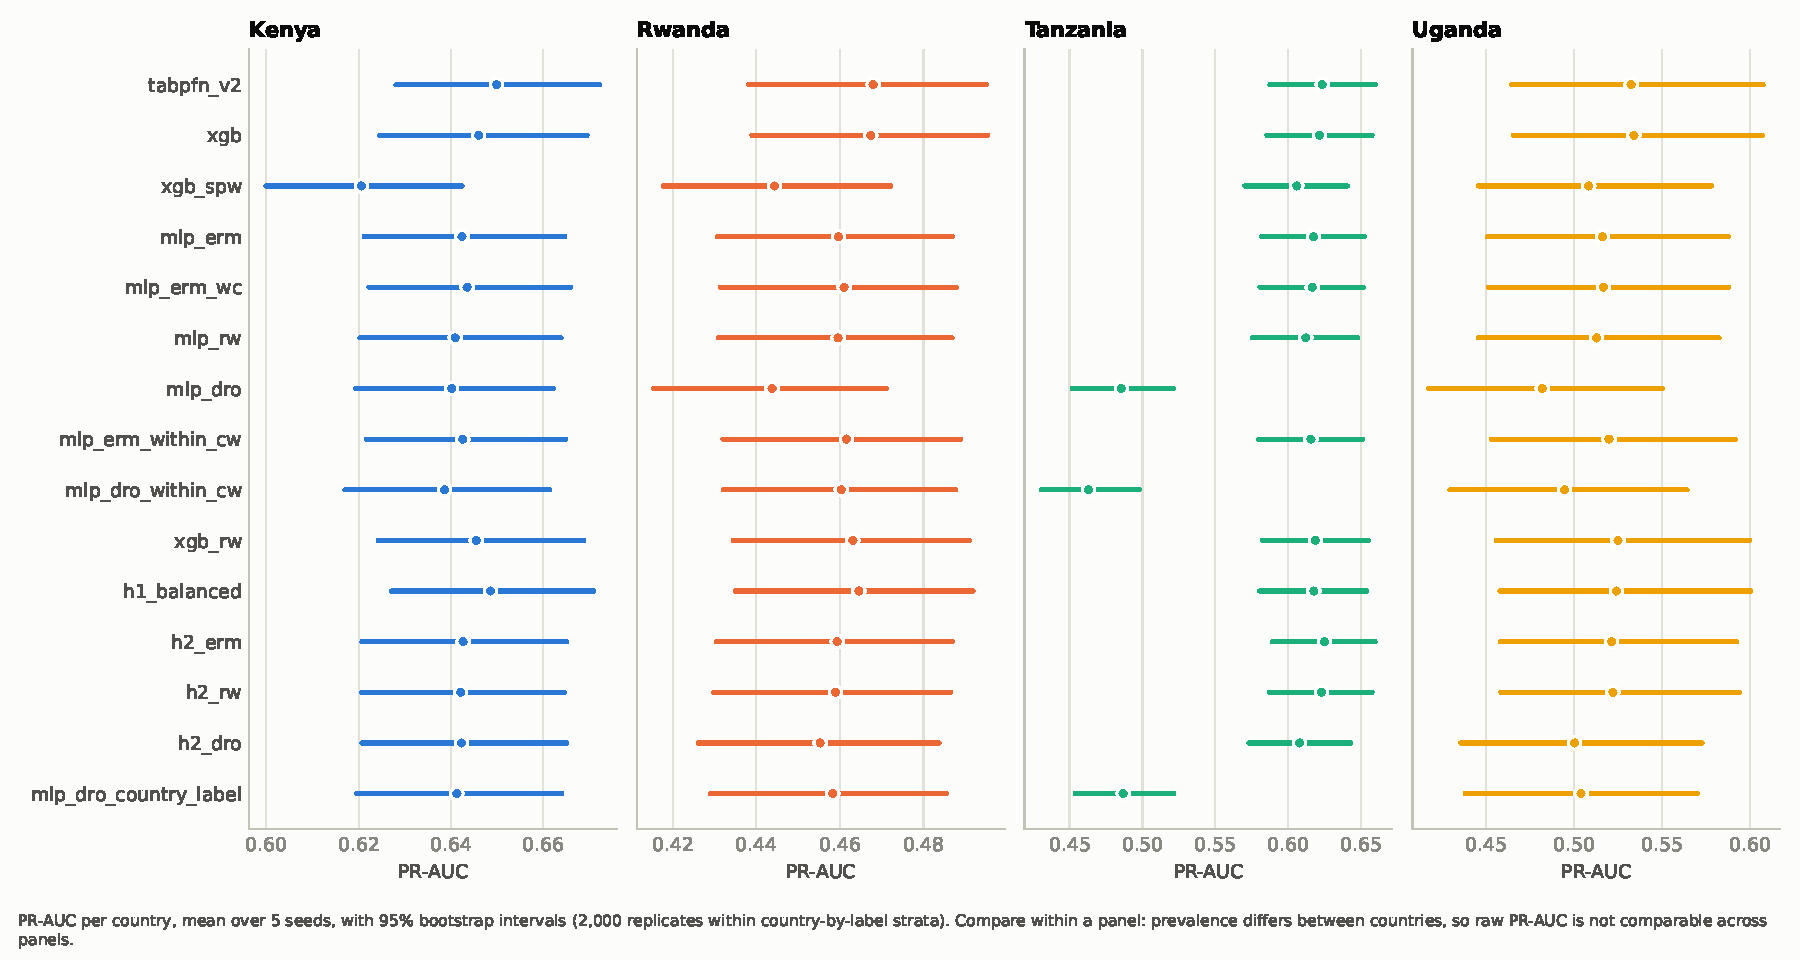
\includegraphics[width=\textwidth]{fig_per_country_prauc.pdf}
  \caption{PR-AUC per country for every within-country arm, five-seed means with 95\% bootstrap intervals. Compare arms within a panel only: prevalence differs between countries.}
  \label{fig:percountry}
\end{figure}

\subsection{RQ3: Group DRO}

\begin{table}[H]
  \centering
  \small
  \caption{Group DRO and its comparators: five-seed means of pooled and per-country PR-AUC.}
  \label{tab:e3}
  \begin{tabular}{lccccc}
    \toprule
    Arm & $P$ & $W$ & Rwanda & Tanzania & Uganda \\
    \midrule
    \arm{mlp\_erm\_wc} (ERM)         & 0.583 & 0.461 & 0.461 & 0.616 & 0.517 \\
    \arm{mlp\_rw} (reweighted)       & 0.580 & 0.460 & 0.460 & 0.612 & 0.513 \\
    \arm{mlp\_dro} (Group DRO)       & 0.543 & 0.444 & 0.444 & \textbf{0.486} & 0.482 \\
    \arm{mlp\_erm\_within\_cw}       & 0.553 & 0.462 & 0.462 & 0.616 & 0.520 \\
    \arm{mlp\_dro\_within\_cw}       & 0.502 & 0.460 & 0.460 & \textbf{0.463} & 0.495 \\
    \arm{mlp\_dro\_country\_label} (E7) & 0.516 & 0.458 & 0.458 & 0.487 & 0.504 \\
    \bottomrule
  \end{tabular}
\end{table}

\begin{table}[H]
  \centering
  \small
  \caption{Paired differences with 95\% bootstrap intervals. Intervals for $W$ can be asymmetric because the worst country can change between replicates.}
  \label{tab:e3paired}
  \begin{tabular}{lcc}
    \toprule
    Comparison & $\Delta W$ & $\Delta P$ \\
    \midrule
    DRO $-$ ERM                                  & $-0.017$ [$-0.036$, $-0.011$] & $-0.040$ [$-0.045$, $-0.034$] \\
    DRO $-$ reweighted                           & $-0.016$ [$-0.033$, $-0.010$] & $-0.037$ [$-0.043$, $-0.032$] \\
    DRO $-$ ERM selected on pooled (sensitivity) & $-0.016$ [$-0.034$, $-0.010$] & $-0.039$ [$-0.044$, $-0.033$] \\
    DRO $-$ ERM, within-country class weights    & $-0.001$ [$-0.041$, $+0.003$] & $-0.051$ [$-0.058$, $-0.044$] \\
    E7 country-by-label $-$ country groups       & $+0.015$ [$+0.003$, $+0.027$] & $-0.027$ [$-0.033$, $-0.023$] \\
    Reweighted $-$ ERM XGBoost                   & $-0.004$ [$-0.009$, $-0.001$] & $-0.002$ [$-0.004$, $-0.000$] \\
    \bottomrule
  \end{tabular}
\end{table}

\textbf{RQ3 is falsified} (Tables~\ref{tab:e3} and~\ref{tab:e3paired}).
\begin{itemize}
  \item \textbf{Criterion 1, within noise:} not met. The gain's interval excludes 0, and $|\text{gain}| = 0.017$ exceeds its seed SD of 0.013. But the gain is negative: Group DRO lowers worst-country PR-AUC.
  \item \textbf{Criterion 2, trivial against cost:} met, since gain $-$ cost $= -0.057 < \delta$.
  \item \textbf{Criterion 3, matched by reweighting:} met, since Group DRO lies entirely below reweighting.
\end{itemize}
Selecting ERM on pooled instead of worst-country PR-AUC gives the same conclusion.

\textbf{Ablations} (Figure~\ref{fig:sweeps}). Worst-country PR-AUC falls as the step size grows: 0.454 at $\eta = 0$, 0.455 at $10^{-3}$, 0.451 at $10^{-2}$, 0.417 at $10^{-1}$ and 0.401 at 1. From $\eta \geq 0.1$, the worst country becomes Tanzania. The adjustment $C$ has no effect, with $W$ between 0.442 and 0.446 for every value. Country-by-label groups (E7) improve on country groups but stay below ERM (0.458 against 0.461), at a pooled cost of 0.067.

\begin{figure}[H]
  \centering
  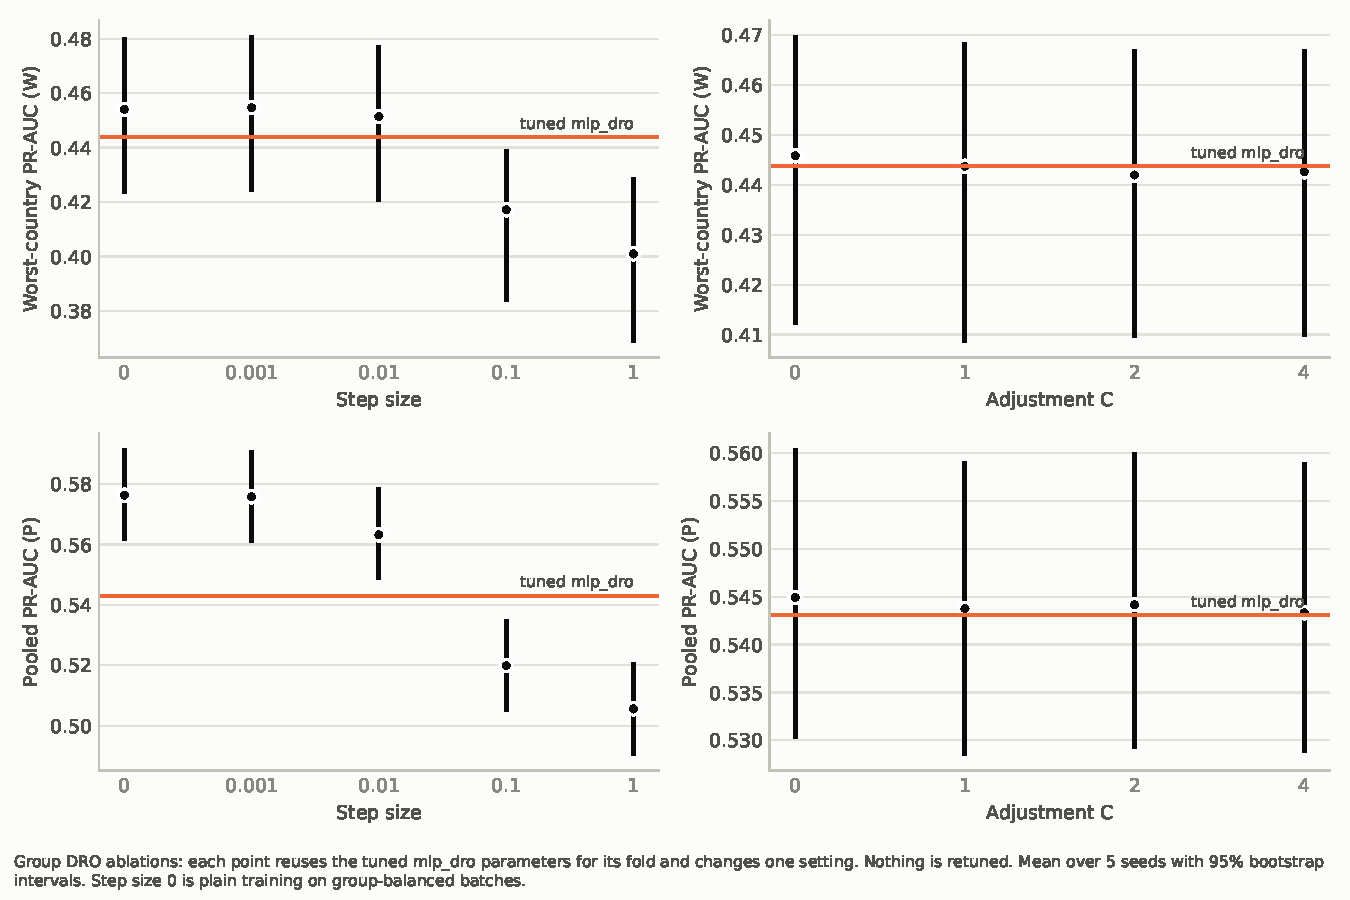
\includegraphics[width=0.85\textwidth]{fig_rq3_sweeps.pdf}
  \caption{Group DRO ablations over step size and adjustment $C$: worst-country (top) and pooled (bottom) PR-AUC. Each point reuses the tuned \arm{mlp\_dro} parameters and changes one setting. Step size 0 is plain training on group-balanced batches.}
  \label{fig:sweeps}
\end{figure}

\textbf{Mechanism} (Figure~\ref{fig:q}). With pooled class weights, $q$ moves steadily towards Kenya, ending at 0.91, against 0.06 for Rwanda and 0.02 each for Tanzania and Uganda. Kenya has the highest training loss throughout (final group loss 0.60, against 0.39 to 0.49 for the others) because it has the highest prevalence. But the worst country by PR-AUC is Rwanda. Group DRO maximises the worst group's \emph{loss}, and here the worst-loss group is not the group with the worst \emph{ranking quality}.

With within-country class weights, $q$ does move to Rwanda (0.65), yet Rwanda's PR-AUC is unchanged (0.460 against 0.462). Both Group DRO variants push Tanzania's weight to almost zero, and Tanzania's PR-AUC collapses, from 0.616 to 0.486 and to 0.463. This collapse accounts for most of Group DRO's pooled cost. It would fit the reversed \texttt{location\_type} relationship described in Section~\ref{sec:experiments}, but we have not tested that explanation.

\begin{figure}[H]
  \centering
  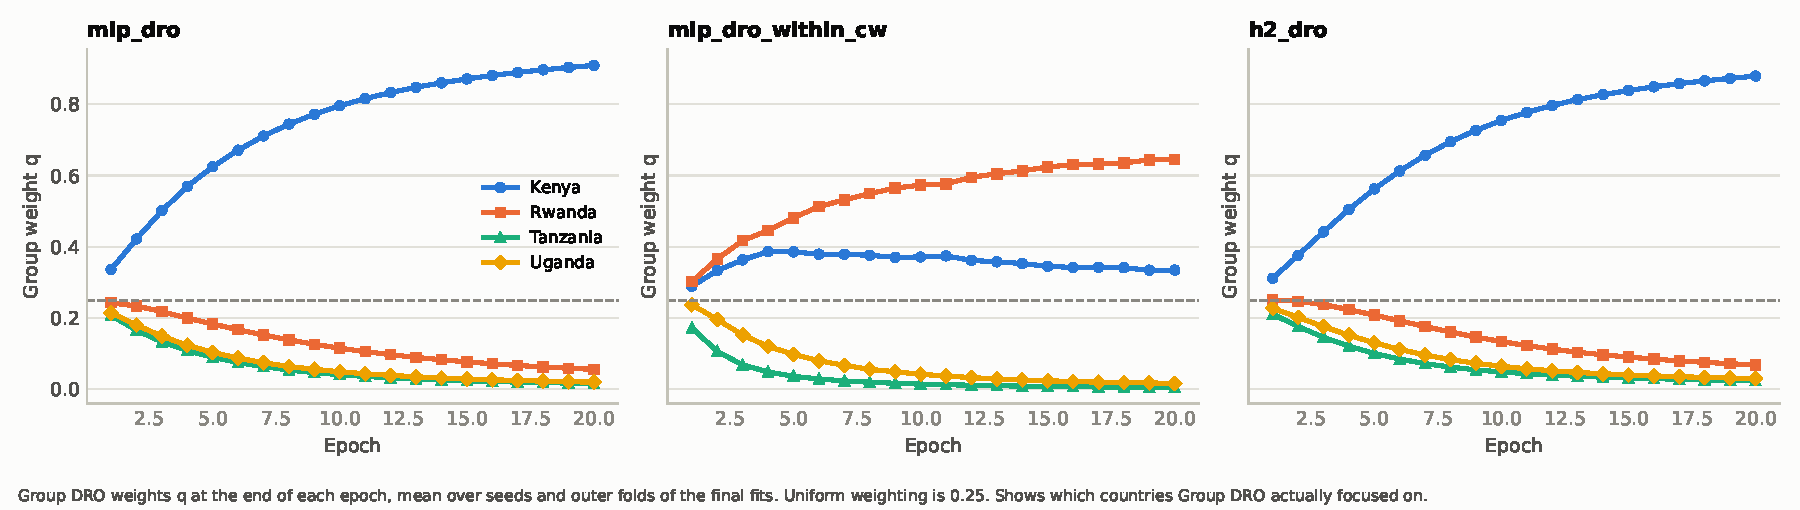
\includegraphics[width=\textwidth]{fig_dro_group_weights.pdf}
  \caption{Group DRO weights $q$ at the end of each epoch, mean over seeds and outer folds. Uniform weighting is 0.25.}
  \label{fig:q}
\end{figure}

\subsection{RQ4: hybrids}

\begin{table}[H]
  \centering
  \small
  \caption{Each hybrid's worst-country PR-AUC against the better of TabPFN and the Group DRO MLP, taken within each bootstrap replicate.}
  \label{tab:e5}
  \begin{tabular}{lccc}
    \toprule
    Hybrid & $W$ & $W(H) - \max\{W(\text{TabPFN}), W(\text{DRO})\}$ & Holm $p$ \\
    \midrule
    H1 \arm{h1\_balanced}   & 0.465 & $-0.003$ [$-0.008$, $-0.001$] & 1.0 \\
    H2 \arm{h2\_rw}         & 0.459 & $-0.009$ [$-0.014$, $-0.004$] & 1.0 \\
    H2 \arm{h2\_dro}        & 0.455 & $-0.013$ [$-0.029$, $-0.008$] & 1.0 \\
    Control \arm{h2\_erm}   & 0.459 & $-0.009$ [$-0.013$, $-0.003$] & -- \\
    \bottomrule
  \end{tabular}
\end{table}

\textbf{RQ4 is falsified} (Table~\ref{tab:e5}). Every hybrid falls below the better of its parents. In the point estimates, that parent is TabPFN, with $W = 0.468$ against 0.444 for the Group DRO MLP.
\begin{itemize}
  \item H1 comes closest. Its loss is inside $\delta$, and it keeps TabPFN's pooled PR-AUC (0.588).
  \item The H2 heads do no better than the ERM-head control.
  \item The Group DRO head inherits the drift towards Kenya, ending at $q = 0.88$ (Figure~\ref{fig:q}).
\end{itemize}

\subsection{RQ5: leave-one-country-out}

\begin{table}[H]
  \centering
  \small
  \caption{PR-AUC on the held-out country, five-seed means. Compare within a row only.}
  \label{tab:e4}
  \begin{tabular}{lccccccc}
    \toprule
    Held out & XGB & MLP & DRO MLP & TabPFN & H1 & H2-rw & H2-DRO \\
    \midrule
    Kenya    & 0.608 & 0.602 & \textbf{0.622} & 0.617 & 0.615 & 0.604 & 0.615 \\
    Rwanda   & 0.388 & 0.386 & \textbf{0.415} & 0.396 & 0.385 & 0.378 & 0.407 \\
    Tanzania & 0.407 & 0.418 & 0.414 & 0.431 & \textbf{0.466} & 0.449 & 0.421 \\
    Uganda   & 0.507 & 0.497 & 0.492 & \textbf{0.513} & 0.509 & 0.501 & 0.498 \\
    \bottomrule
  \end{tabular}
\end{table}

\textbf{RQ5 is falsified} (Table~\ref{tab:e4}, Figure~\ref{fig:loco}). No method is consistently better, and every method is clearly beaten after Holm correction in at least one held-out country.
\begin{itemize}
  \item \textbf{Tanzania:} H1 has the only clear win over all six other methods.
  \item \textbf{Rwanda:} the Group DRO MLP clearly beats five of six methods, but is not separated from H2-DRO (Holm $p = 0.14$).
  \item \textbf{Kenya and Uganda:} no clear winner. Uganda's intervals are about $\pm 0.07$ wide.
\end{itemize}

Compared with within-country cross-validation, held-out PR-AUC drops by 0.03--0.04 in Kenya, 0.07--0.08 in Rwanda and 0.15--0.21 in Tanzania. In Uganda the drop is 0.00--0.03, and every interval includes 0. Group DRO has the smallest drop in every country (0.018, 0.029, 0.072 and $-0.010$), but its within-country scores were lower to begin with, notably in Tanzania. Following \citet[p.~17]{koh2021wilds}, we do not read these drops as pure shift, because training size also differs and a country may be intrinsically harder.

\begin{figure}[H]
  \centering
  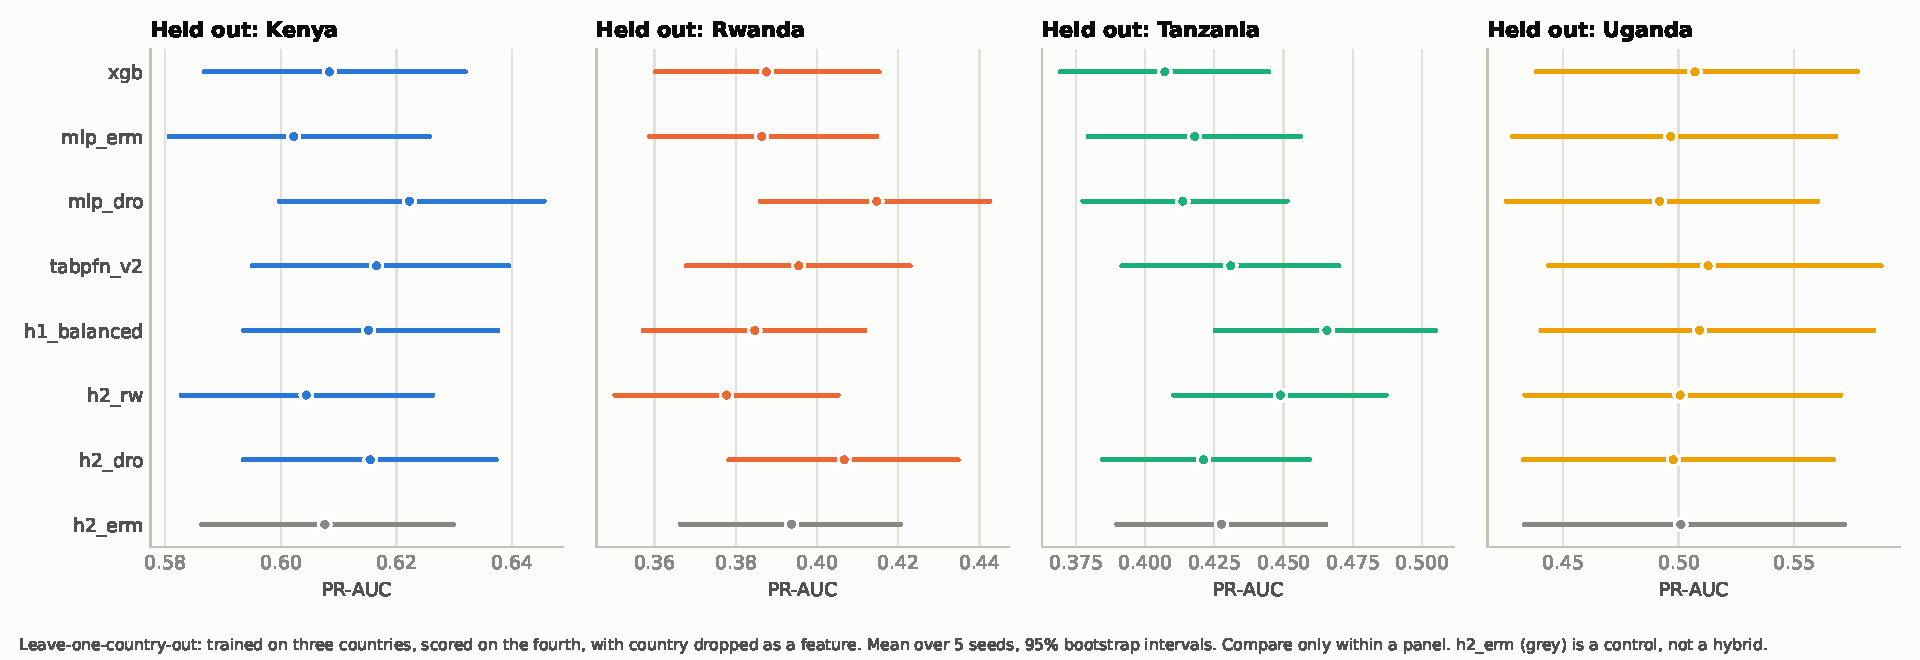
\includegraphics[width=\textwidth]{fig_rq5_loco.pdf}
  \caption{Leave-one-country-out PR-AUC with 95\% bootstrap intervals. \arm{h2\_erm} (grey) is a control, not a hybrid.}
  \label{fig:loco}
\end{figure}

\subsection{RQ6: explanations}

\begin{table}[H]
  \centering
  \small
  \caption{Disagreement in feature rankings beyond resampling noise ($1 - \rho_{\text{Spearman}}$), mean and 95\% interval over 200 size-matched draws. Kendall $\tau$ gives the same reading.}
  \label{tab:e6}
  \begin{tabular}{lc}
    \toprule
    Quantity & Cross-country minus noise \\
    \midrule
    XGBoost (primary)           & 0.038 [0.033, 0.042] \\
    ERM MLP                     & 0.034 [0.028, 0.040] \\
    Group DRO MLP               & 0.009 [0.000, 0.021] \\
    Group DRO $-$ ERM, in Rwanda & 0.007 [$-0.017$, $+0.025$] \\
    \bottomrule
  \end{tabular}
\end{table}

\textbf{RQ6 is not falsified for the primary model} (Table~\ref{tab:e6}, Figure~\ref{fig:shap}). For XGBoost and the ERM MLP, feature rankings differ between countries by more than two random halves of one country do. The excess is small, though. \texttt{cellphone\_access} and \texttt{education\_level} are the two most-relied-on features in every country for every model, and the differences lie further down the ranking. For example, XGBoost relies on \texttt{location\_type} less in Tanzania than in the other three countries. For the Group DRO MLP, the interval's lower bound is 0, which counts as including 0. In Rwanda, Group DRO does not change which features matter beyond noise.

\textbf{Caveat on the MLP rows.} The MLPs were refitted for E6 with 32 CPU threads, while their training runs had used 5. MLP training is deterministic only at a fixed thread count. On our hardware, changing it moved scores by up to 0.049 (mean 0.009). The MLP attributions therefore explain models with the same data, hyperparameters and seed as the evaluated ones, but a different floating-point path. Their largest per-fold score difference from the saved predictions was 0.02 to 0.17. The XGBoost refits matched to $3 \times 10^{-8}$.

\begin{figure}[H]
  \centering
  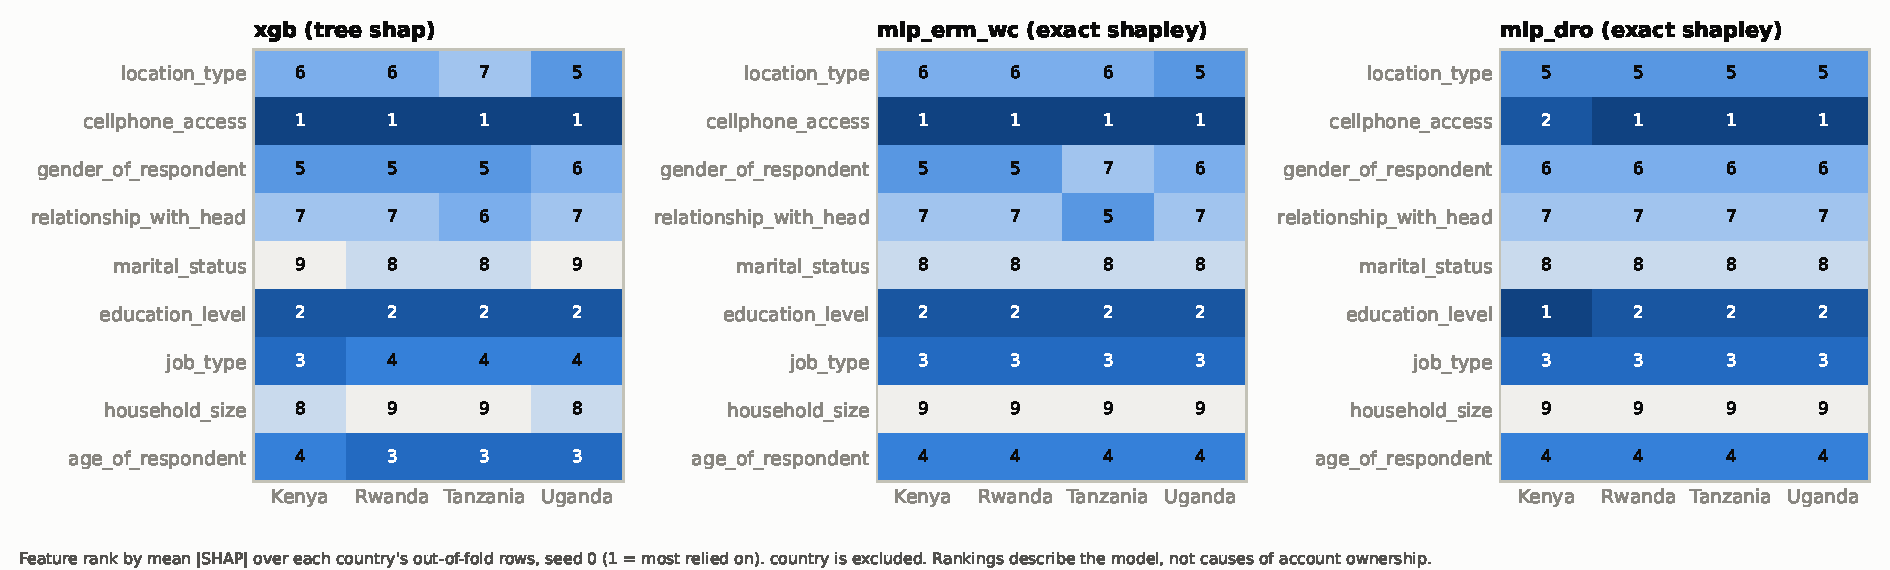
\includegraphics[width=\textwidth]{fig_e6_rankings.pdf}
  \caption{Feature rank by mean absolute SHAP over each country's out-of-fold rows, seed 0 (1 = most relied on). \texttt{country} is excluded.}
  \label{fig:shap}
\end{figure}

% 6. Discussion
\section{Discussion}
\label{sec:discussion}

\paragraph{The limit lies in the data, not the model.} Across 24 within-country model variants, worst-country PR-AUC lies between 0.40 and 0.47. Excluding the deliberately extreme step-size ablations, it lies between 0.44 and 0.47. The gap $G$ is 0.12 for every model trained with pooled class weights and without Group DRO. Where the gap is smaller, it is because pooled PR-AUC fell, not because the worst country improved. Rwanda remained the worst country for every one of these approaches: a foundation model pretrained on millions of synthetic tasks, a tuned tree ensemble, reweighting, an objective that targets Rwanda directly, and a TabPFN context with equal country shares. This matches the observation in WILDS that a worst-group gap can reflect intrinsic difficulty, which more attention to that group does not fix \citep[pp.~113--115]{koh2021wilds}. Rwanda is not a small group: it has the most rows and the second-highest prevalence. Our reading is that these ten survey features separate account holders from non-holders less well in Rwanda than elsewhere. We have not tested why.

\paragraph{Why Group DRO failed.} First, it weights groups by training loss, and log-loss is highest in the highest-prevalence group. A mini-max objective on loss is therefore not a mini-max objective on a ranking metric when prevalence differs between groups. We found no discussion of this point in the literature we reviewed. Second, correcting the target did not help: within-country class weights moved the weight to Rwanda without moving Rwanda's PR-AUC, and the cost fell on Tanzania, which the objective then ignored. This mirrors \citet{koh2021wilds} and \citet{stahlschmidt2024domain}, and our pre-registration noted it in advance as a plausible outcome.

\paragraph{TabPFN as a practical result.} Untuned TabPFN v2 matched tuned XGBoost within 0.003 PR-AUC in about 3~s per fold. This agrees with independent clinical benchmarks \citep{shaktah2026established}. Pretraining did not supply fairness, consistent with \citet{liu2026causal} and \citet[pp.~22--23]{kurashkin2026current}.

\paragraph{Exploratory observations.} The following patterns were seen after the results and were not pre-registered.
\begin{itemize}
  \item \textbf{H1 when Tanzania is held out.} Equal country shares in the context gave a clear win (0.466 against 0.431 for TabPFN's default context). This suggests context composition matters most when the target country's feature relationships differ from the training countries', in line with the view that context is now a design lever \citep[p.~19]{kurashkin2026current}.
  \item \textbf{Group DRO under shift.} Group DRO was the strongest method when Kenya or Rwanda was held out, despite being the weakest model within countries. Part of this is mechanical, and a pre-registered test is needed.
\end{itemize}

\paragraph{Uganda is not the worst-off country.} The study framework expected Uganda, which has the smallest sample and the lowest prevalence. Uganda was the worst country in only one seed of one ablation. Its intervals are also wide, so this study can say little about Uganda specifically. Fixing the analysis on Uganda in advance would have measured the wrong group.

\paragraph{Practical implications.} If the aim is to reach the unbanked in the worst-served country, our results point to better information about that country rather than a different model or objective. Examples are features capturing mobile money, documentation or distance, which Findex reports as barriers \citep[pp.~53--54]{demirguckunt2022findex}. This is our inference and was not tested. A better classifier also does not by itself produce inclusion: free accounts alone had no measurable welfare effect in Uganda \citep[p.~28]{demirguckunt2022findex}.

\paragraph{Limitations.}
\begin{itemize}
  \item \textbf{Confounding.} Country is confounded with survey year.
  \item \textbf{Label.} \texttt{bank\_account} excludes mobile money, the main route to account ownership in East Africa \citep[p.~20]{demirguckunt2022findex}; \citep{engelmann2018unbanked}.
  \item \textbf{Uncorrected data anomalies.} The coding of Tanzania's \texttt{location\_type} and the country-specific \texttt{job\_type} levels were left as they are. Both may affect leave-one-country-out results.
  \item \textbf{TabPFN context.} TabPFN read stratified contexts of about 10,000 rows, not the whole training fold, and ran in fp16. The measured effect of fp16 on scores was at most 0.004.
  \item \textbf{Tuning.} Budgets follow the earlier baseline: 15 trials for XGBoost and 8 for the MLPs, with Group DRO searching two more hyperparameters in the same 8 trials. All models trained for 20 epochs without early stopping, although Group DRO is said to work best before training loss vanishes \citep[p.~67]{koh2021wilds}.
  \item \textbf{Leave-one-country-out tuning} used inner folds within the training countries, so model selection was not itself shift-aware.
  \item \textbf{H2 tuning.} Inner-loop embeddings may carry inner-validation labels through the context. This does not affect the outer test rows.
  \item \textbf{Worst-country estimate.} The floating minimum is biased downward for small groups.
  \item \textbf{Explanations.} E6 uses a single seed, and its MLP attributions come from refitted models, as described above.
  \item \textbf{Group DRO source.} Group DRO's update rule is given as our own statement, because its usual source was not in our literature.
\end{itemize}

\paragraph{Ethics.} The data are survey responses about individuals. A model that ranks people by their probability of holding a bank account could support outreach, but it could also support exclusion or targeted marketing. The consumer risks Findex reports in Uganda and Kenya \citep[pp.~150, 172]{demirguckunt2022findex} apply to whatever follows outreach. No model here is fit for decisions about individuals.

% 7. Conclusion
\section{Conclusion}

Neither route improved prediction for the worst-off country.
\begin{itemize}
  \item TabPFN v2 matched tuned XGBoost without tuning but left the gap unchanged.
  \item Group DRO made the worst country worse. It optimised for the highest-loss country, Kenya, rather than the lowest-PR-AUC country, Rwanda, and when redirected to Rwanda it still did not help.
  \item The hybrids did not beat their parents.
  \item No method was consistently best when a country was held out.
\end{itemize}
Worst-country PR-AUC stayed between 0.44 and 0.47 across every model family and objective, apart from the extreme step-size ablations. For this task, the limit on serving the worst-off country appears to lie in the data rather than in the choice of model or objective.

Future work could:
\begin{itemize}
  \item test a group-robust objective defined on a ranking metric rather than on loss;
  \item test the Tanzania coding hypothesis directly;
  \item run a pre-registered test of the leave-one-country-out patterns;
  \item add features that reflect mobile money and access barriers.
\end{itemize}

% 8. Acknowledgments
\section*{Acknowledgments}
TabPFN v2 weights are used under the Prior Labs License 1.1.

% ------------------------------------------------
% References
% ------------------------------------------------
\bibliographystyle{IEEEtranN}
\bibliography{references}

% ------------------------------------------------
% Appendices
% ------------------------------------------------
\clearpage
\appendix
\section*{Appendix}
\addcontentsline{toc}{section}{Appendix}
\setcounter{section}{1}
\setcounter{table}{0}
\renewcommand{\thetable}{A\arabic{table}}

\subsection{Experiment completion status}

Table~\ref{tab:status} records which of the planned experiments were completed.

\begin{table}[H]
  \centering
  \small
  \caption{Completion status of every planned experiment.}
  \label{tab:status}
  \begin{tabular}{p{0.45\textwidth}p{0.45\textwidth}}
    \toprule
    Experiment & Status \\
    \midrule
    E1 baseline reproduction & Completed; exact reproduction \\
    E2 main benchmark & Completed; 5 seeds $\times$ 5 folds \\
    E3 Group DRO, reweighting, ablations, within-country pair & Completed \\
    E4 leave-one-country-out, including all hybrids & Completed \\
    E5a H1; E5b H2 with three heads & Completed \\
    E5c H3, fine-tuning TabPFN with Group DRO & \textbf{Not completed}; infeasible with the installed package \\
    E6 SHAP & Completed for seed 0; MLP refit caveat; TabPFN not explained \\
    E7 country-by-label groups & Completed \\
    \bottomrule
  \end{tabular}
\end{table}

No hypothesis, rule, arm or setting was changed after results were seen. The within-country class-weight pair was added before any result existed.

% ------------------------------------------------
% Document Ends
% ------------------------------------------------
\end{document}
